\documentclass[]{article}
\usepackage[hyphens]{url}
\usepackage[pdfusetitle,colorlinks,plainpages]{hyperref}
\usepackage[dutch]{babel}
\usepackage{lipsum} % for dummy text only
\usepackage{csquotes}
\usepackage[backend=bibtex]{biblatex}
%\usepackage[acronym]{glossaries}
\usepackage{eurosym}
\usepackage{subfigure}
\usepackage{multirow}
\usepackage{tikz}
\usepackage{listings}
\usepackage{caption}
\usepackage{pdfpages}

\usepackage{todonotes}
\usepackage{placeins}

\usepackage{tikz}
\usepackage{pgfplots}
\usepackage{verbatim}

%opening
\title{IMP: HBase}
\author{Thomas Uyttendaele}

\begin{document}

\maketitle

\section{Algemene inleiding}
In deze sectie zal voor de verschillende systemen de automatisering van installatie en configuratie met behulp van IMP uitgelegd worden. Er zal steeds de afhankelijkheden gegeven worden, een domeinmodel, uitleg bij het domeinmodel en voorbeeld configuratie gegeven worden. 

De automatisatie van installatie is ontwikkeld en getest met Fedora 18 en 20, op andere distributies en versies is er niet getest. 
Elk systeem maakt gebruik van \textit{ip::services::Server}, een instantie hiervan is een (virtuele) machine met een IP adres en besturingssysteem. 

Bij elke instantie is het verplicht om de firewall uit te zetten en SELinux op permissive te zetten. Dit kan met behulp van de volgende commando's: 
\begin{lstlisting}[frame=single, breaklines=true]
systemctl stop firewalld.service  
systemctl disable firewalld.service  
setenforce 0
sed -i "s/SELINUX=enforcing/SELINUX=permissive/g" /etc/sysconfig/selinux
sed -i "s/SELINUX=enforcing/SELINUX=permissive/g" /etc/selinux/config|
\end{lstlisting}

\section{HBase}
\textit{Link: \url{https://github.com/thuys/hbase}}

Benodigde IMP modules: std, net, ip, redhat, hosts en yum. 

De installatie en configuratie is gebeurd aan de hand van de uitleg en yum-repository van Cloudera\footnote{\url{http://www.cloudera.com/content/cloudera-content/cloudera-docs/CDH4/4.2.0/CDH4-Installation-Guide/CDH4-Installation-Guide.html}}. 

\subsection{Domein model en uitleg}
Het domeinmodel is te zien in figuur \ref{fig:imp-hbase-domeinmodel}.

\paragraph{HBaseMaster} Dit is de implementatie van de HMaster, dient toegewezen worden aan een host met java installatie. De poort is de poort waarop de HMaster actief is. 
 
\paragraph{HRegion} Dit is de implementatie van de HRegionServer, dient toegewezen worden aan een host met java installatie. De poort is de poort waarop de HRegionServer actief is. 

\paragraph{HadoopHDFS} Dit is de implementatie van de HDFS namenode, dient toegewezen worden aan een host met java installatie. De poort is de poort waarop de namenode actief is, de directory is de directory voor HBase  en de nameDir de lokatie waar de data op harde schijf weggeschreven zal worden. 

\paragraph{HadooDatapHDFS} Dit is de implementatie van de HDFS datanode, dient toegewezen worden aan een host met java installatie. De poort is de poort waarop de namenode datanode is, de directory is de directory voor HBase en de dataDir de lokatie waar de data op harde schijf weggeschreven zal worden. 

\paragraph{Zookeeper} Dit is de implementatie van een enkele Zookeeper. Bij het toewijzen van meerdere aan een cluster zullen de Zookeepers een cluster vormen. 

\paragraph{Javahost} Dit is een server waar Java is op geïnstalleerd. 

\begin{figure}[ht!]
\centering
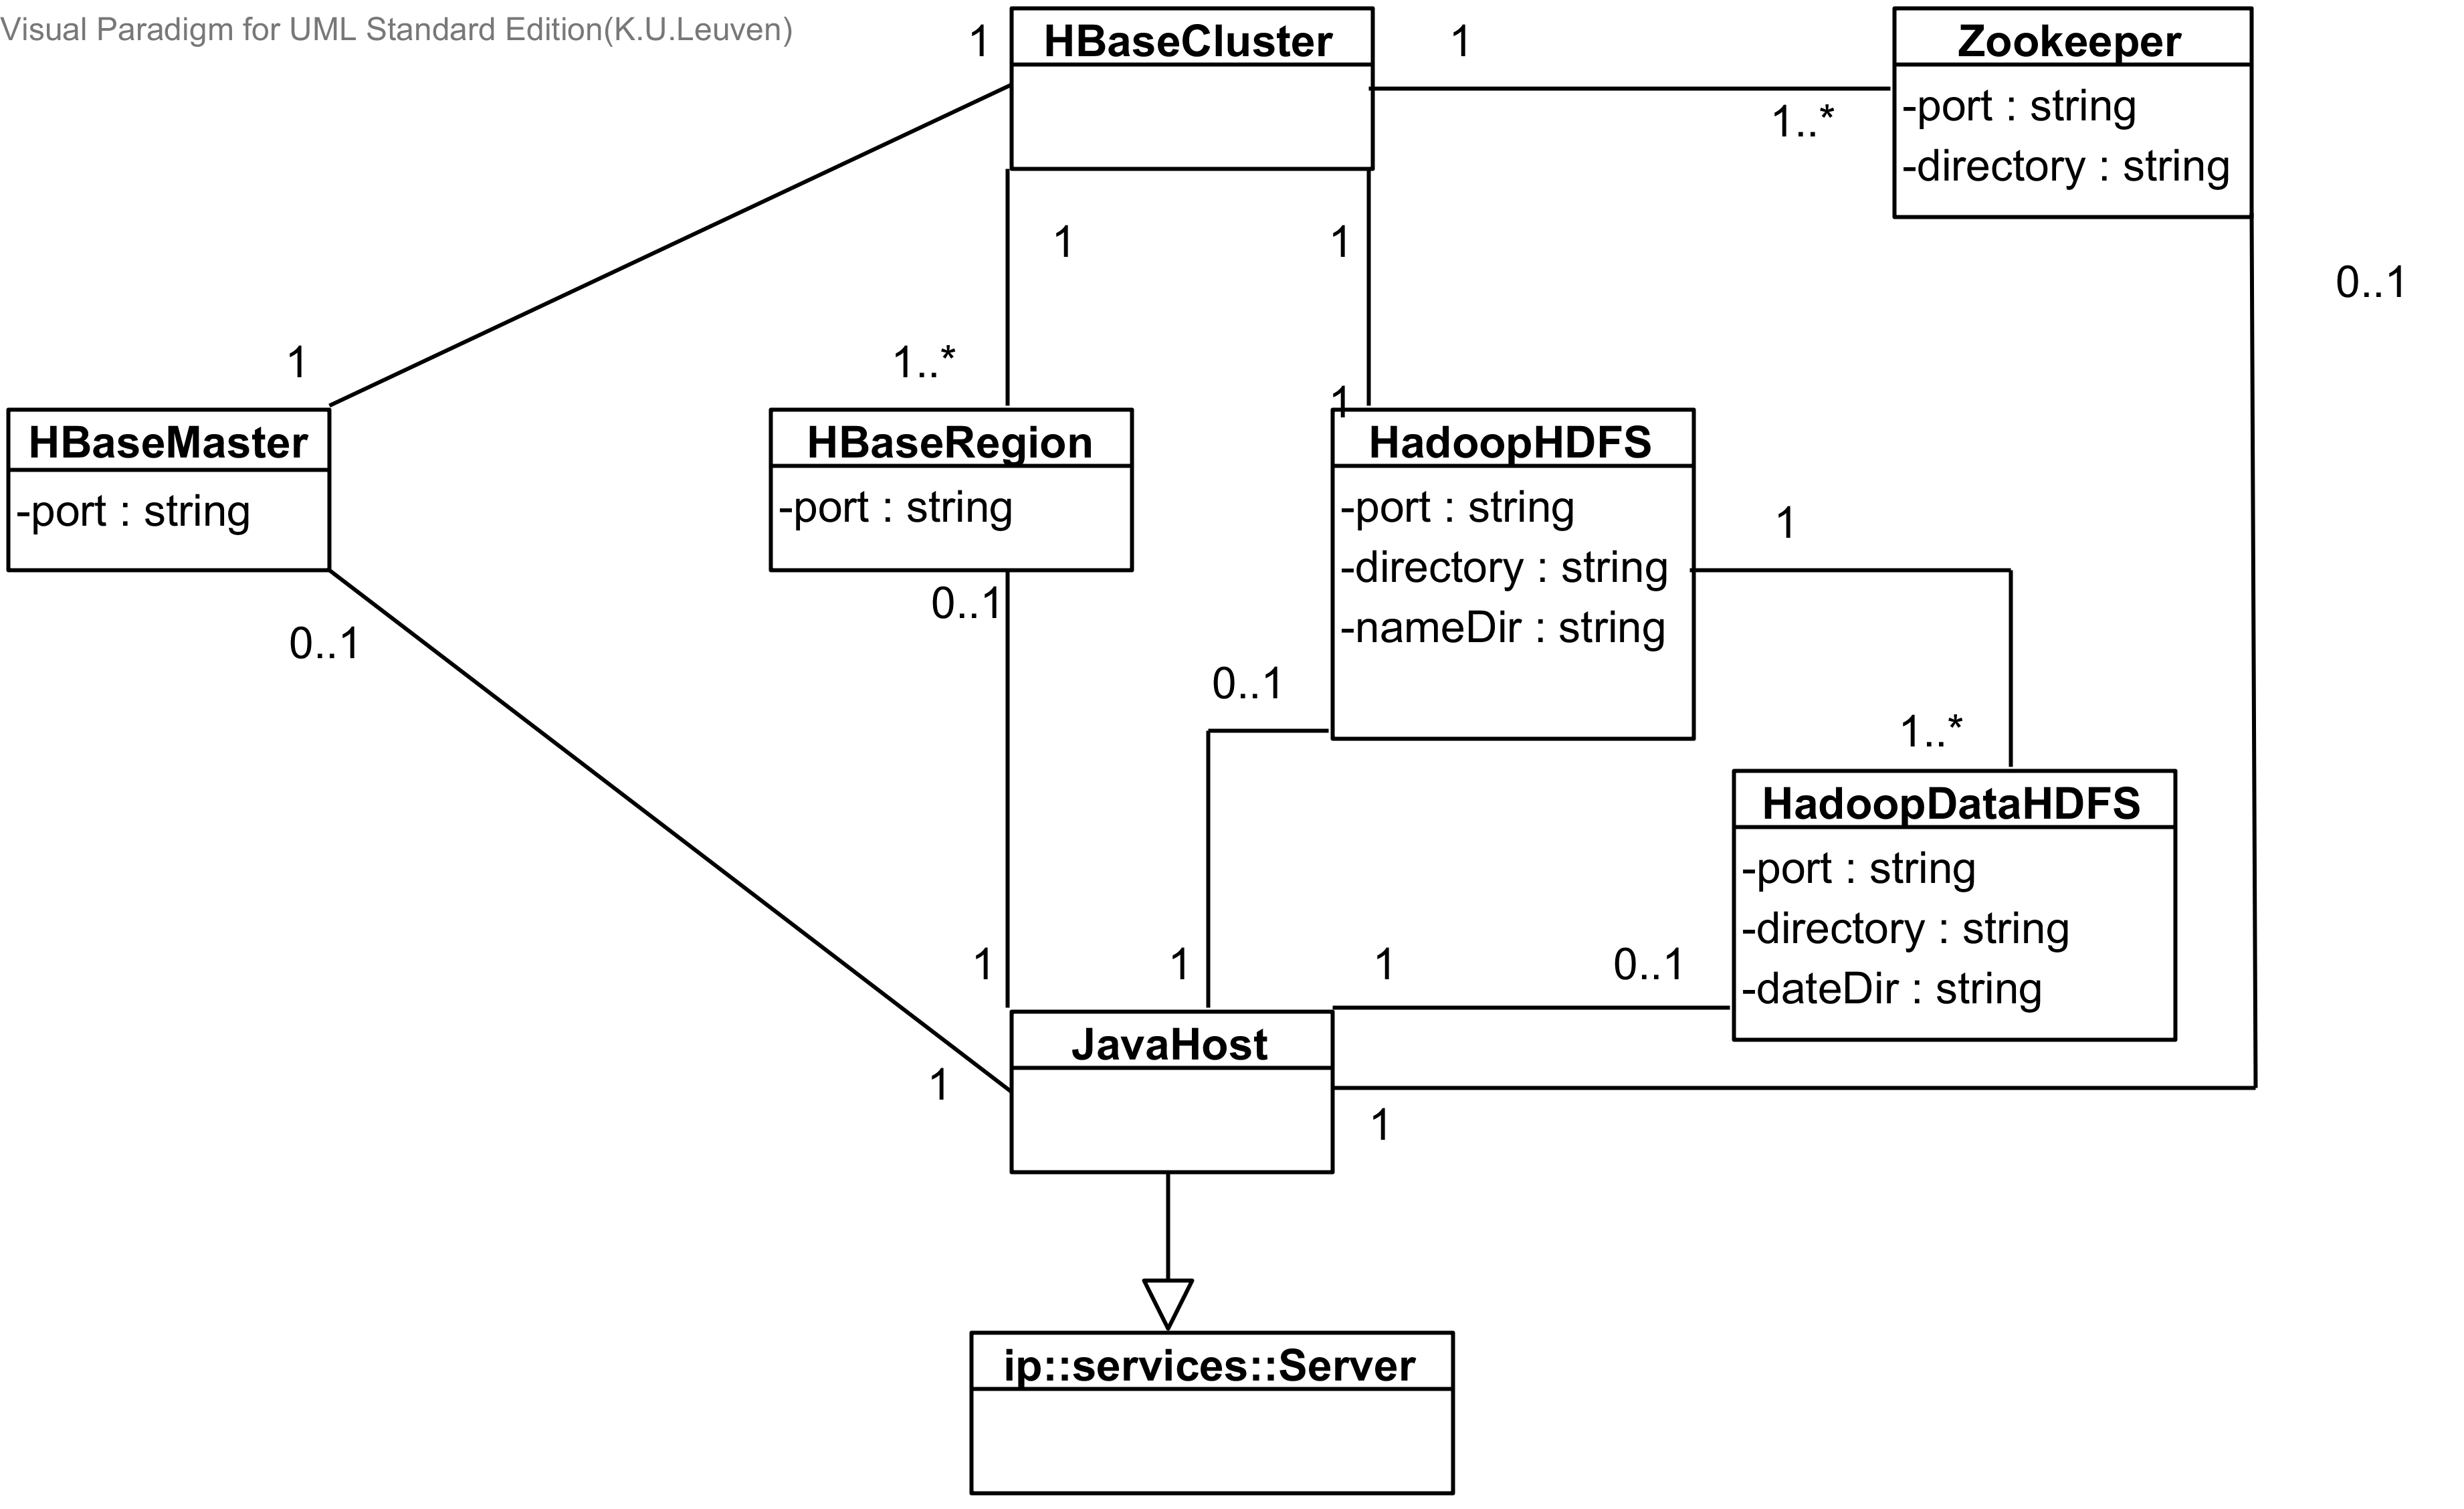
\includegraphics[width=\linewidth]{img/HBase-Domeinmodel.png}
\caption{HBase: Domeinmodel HBase in IMP}
\label{fig:imp-hbase-domeinmodel}
\end{figure}

\subsection{Voorbeeld configuratie}
De configuratie voor de testomgeving gaat als volgt: 

\lstinputlisting[language=Python, breaklines=true, frame=single]{code/imp-hbase.conf}

\end{document}
